\documentclass[conference]{IEEEtran}

\usepackage[usenames,dvipsnames,svgnames,table]{xcolor}
\usepackage{amsmath}
\usepackage{amsfonts}
\usepackage{cite}
\usepackage{graphicx}
\usepackage{listings}
\usepackage{multirow}
\usepackage{tabularx}
\usepackage{varioref}
\usepackage{hyperref}
\usepackage[noabbrev,capitalize]{cleveref}
\usepackage[group-separator={,}, group-four-digits=true]{siunitx}
\usepackage{lscape}
\usepackage{bm}
\usepackage{chngpage}
\usepackage{blindtext} % For filler text

\usepackage[english]{babel}
\usepackage[utf8]{inputenc}

%Includes "References" in the table of contents
\usepackage[nottoc]{tocbibind}


\lstset{
  frame=single,
  basicstyle=\ttfamily,% print whole listing small
  language=R,
  aboveskip=3mm,
  belowskip=3mm,
  showstringspaces=false,
  columns=flexible,
  numbers=none,
  commentstyle=\color{ForestGreen},
  stringstyle=\color{Maroon},
  breaklines=true,
  breakatwhitespace=true,
  tabsize=2,
  literate={<-}{{$\gets$}}1 {~}{{$\sim$}}1
}

\hypersetup{
  colorlinks=true,
  linkcolor=blue,
  urlcolor=blue,
}

\sisetup{output-exponent-marker=\textsc{e}}

\begin{document}

\title{Machine Learning Final Project}
\author{
\IEEEauthorblockN{William Clark}
\IEEEauthorblockA{will.clark@chicagobooth.edu\\
University of Chicago Booth School of Business}
\and
\IEEEauthorblockN{Matthew DeLio}
\IEEEauthorblockA{mdelio@chicagobooth.edu\\
University of Chicago Booth School of Business}}

\maketitle

\section{Summary}

\section{Modelling}
\subsection{Facial Keypoints Introduction}
\subsection{Building a Model (Tools \& Software)}
\subsection{Initial Models}
\subsection{Individual Feature Models}
Dropout, l1/l2 regularization, and momentum/learning rate.
\subsection{Missing Feature Model}
Since the data contain many missing features caused by partially obscured images, our resulting model must also predict the presence of features.  To predict this we turn to a slightly modified version with a sigmoid non-linearity on the output layer and the binary cross-entropy loss function defined in \cref{eq:bin_cross}.

\[\label{eq:bin_cross}
 L = -target \log(p) - (1 - target) \log(1 - p)
\]

For many of the features, the neural network does a good job separating the classes and producing probabilities that make logical sense.  The ones that it doesn't separate well, like \texttt{Left Eye Center}, \texttt{Right Eye Center} and \texttt{Mouth Center Bottom Lip}, have few missing data-point exemplars in the training data (7, 9, 22 respectively out of 4934).

\begin{figure}[!ht]
  \centering
  \caption{Boxplots for Missing Eye Features}
  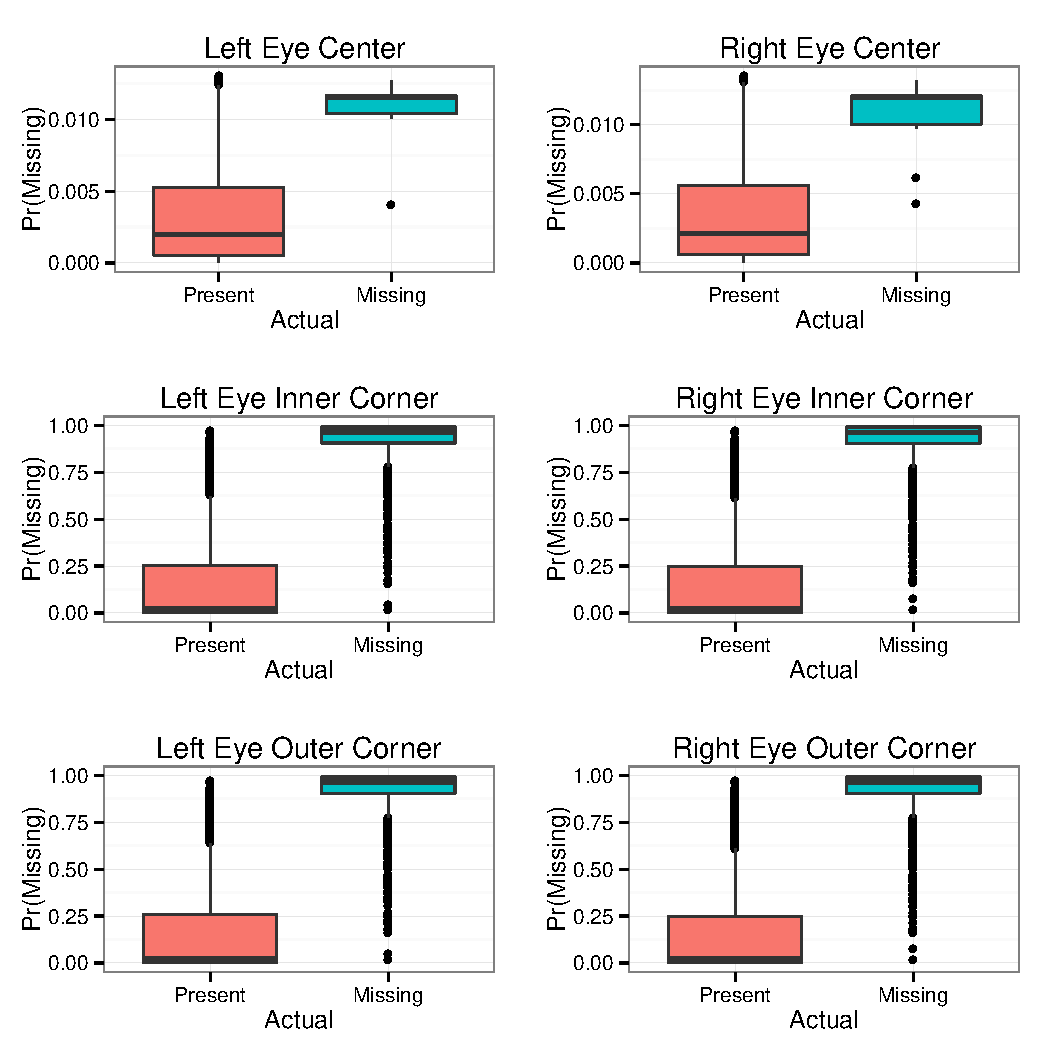
\includegraphics[scale=.5]{logistic_boxplots_eye.pdf}
  \label{fig:logistic_boxplots_eye}
\end{figure}

\begin{figure}[!ht]
  \centering
  \caption{Boxplots for Missing Eyebrow Features}
  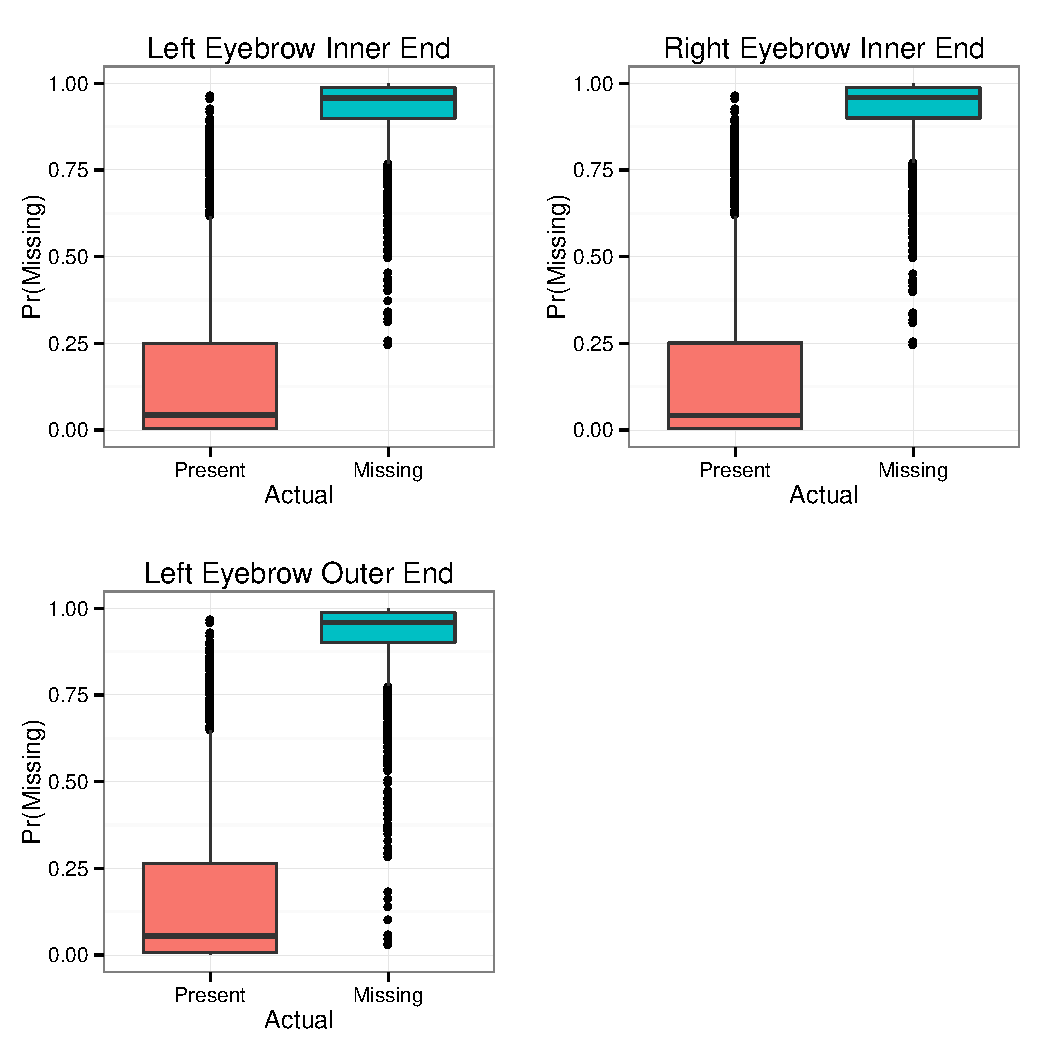
\includegraphics[scale=.5]{logistic_boxplots_eyebrow.pdf}
  \label{fig:logistic_boxplots_eyebrow}
\end{figure}

\begin{figure}[!ht]
  \centering
  \caption{Boxplots for Missing Mouth Features}
  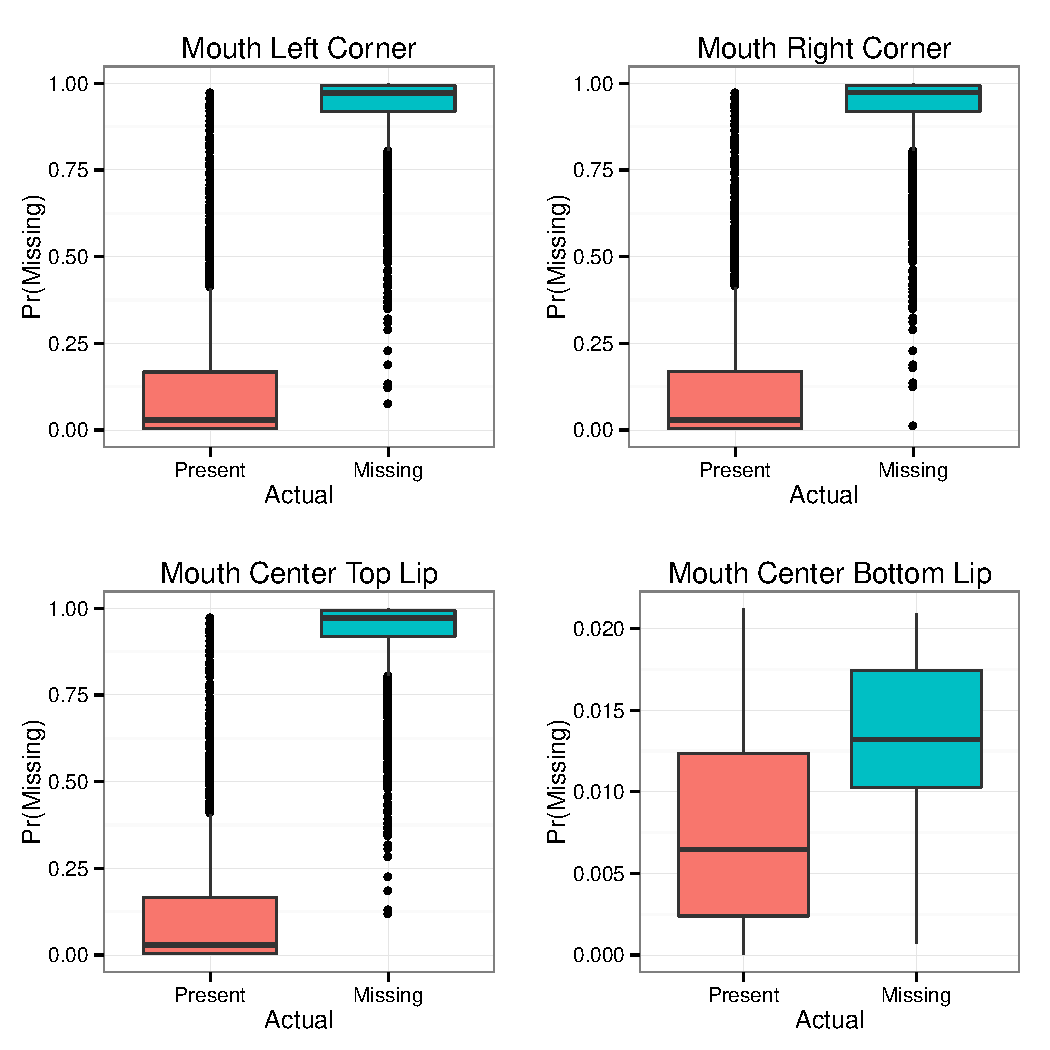
\includegraphics[scale=.5]{logistic_boxplots_mouth.pdf}
  \label{fig:logistic_boxplots_mouth}
\end{figure}

\begin{figure}[!ht]
  \centering
  \caption{Boxplots for Missing Nose Feature}
  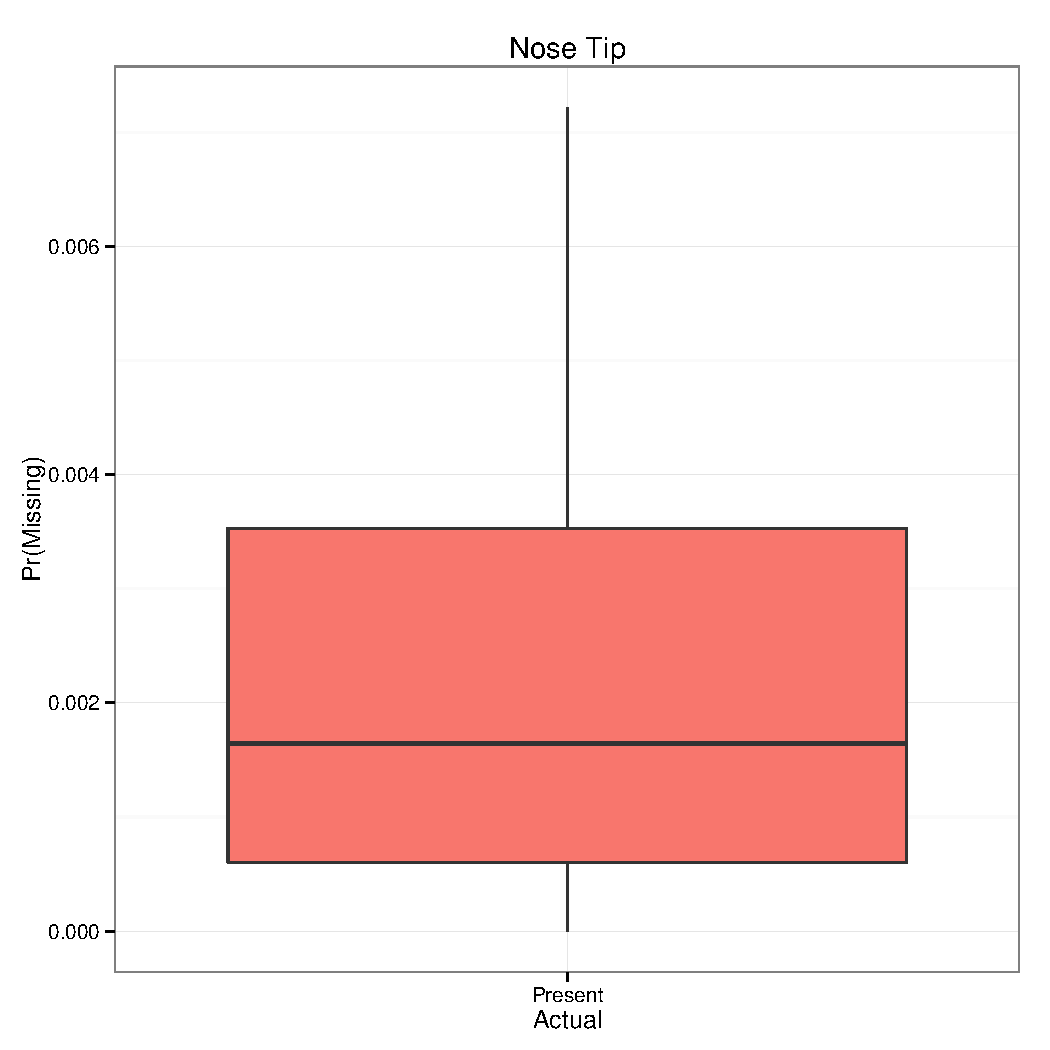
\includegraphics[scale=.5]{logistic_boxplots_nose.pdf}
  \label{fig:logistic_boxplots_nose}
\end{figure}

With the output trained, we next turn to determining the optimal cutoff.  Using the R package \texttt{OptimalCutpoints} we choose to maximize the accuracy area (Lewis et al. 2008; Greiner 1995, 1996) which is defined in \cref{eq:roc_aa}.

\[\label{eq:roc_aa}
AA(c)=\frac{TP(c)TN(c)}{(TP(c)+FN(c))(FP(c)+TN(c))}
\]
where $TP$ = True Positives, $TN$ = True Negatives, $FN$ = False Negatives, \& $FP$ = False Positives



Show boxplots, ROC curves.
\subsection{Combined Loss Model}
Semi-failed attempt to train missing signals and coordinates simultaneously.
\subsection{Putting It All Together}
Show examples

\section{Kaggle Submission}
Ranking?

\section{Applications}
\begin{enumerate}
\item Engagement Detection
\end{enumerate}

\end{document}

% \input{.tex}

% \begin{figure}[!htb]
%   \centering
%   \begin{subfigure}[b]{0.49\textwidth}
%     \caption{}
%     \includegraphics[width=\textwidth]{.pdf}
%     \label{fig:}
%   \end{subfigure}
%   \hfill
%   \begin{subfigure}[b]{0.49\textwidth}
%     \caption{}
%     \includegraphics[width=\textwidth]{.pdf}
%     \label{fig:}
%   \end{subfigure}
%   \caption{}
% \end{figure}

% \begin{figure}[!htb]
%   \centering
%   \caption{}
%   \includegraphics[scale=.5]{.pdf}
%   \label{fig:}
% \end{figure}